\subsection{Scaling Study for GPU using CUDA}
\label{subsec:gpu-cuda-study}
% Identify configurations that are particularly good and particularly bad. Using your knowledge of this GPU device, as well as any results you observed from ncu reports of the Achieved Occupancy % and % of peak sustained memory bandwidth metrics, explain why the good performers are doing so well, and explain why the poor performers are not doing so well. 
% You may wish to consult the A100 architecture whitepaper, which has useful information about the Ampere A100 platform.
The objective of this experiment is to analyze performance variations across different configurations of thread block counts and threads per block to identify the optimal configurations for achieving better GPU performance.

As shown in Figure~\ref{fig:runtime_heatmap}, runtime performance is significantly poorer with smaller thread block counts or lower threads-per-block configurations. In contrast, configurations using larger block sizes and higher thread counts per block yield notably improved runtimes. This pattern suggests that runtime efficiency is highly correlated with the total number of threads.

\begin{figure}[htbp]
    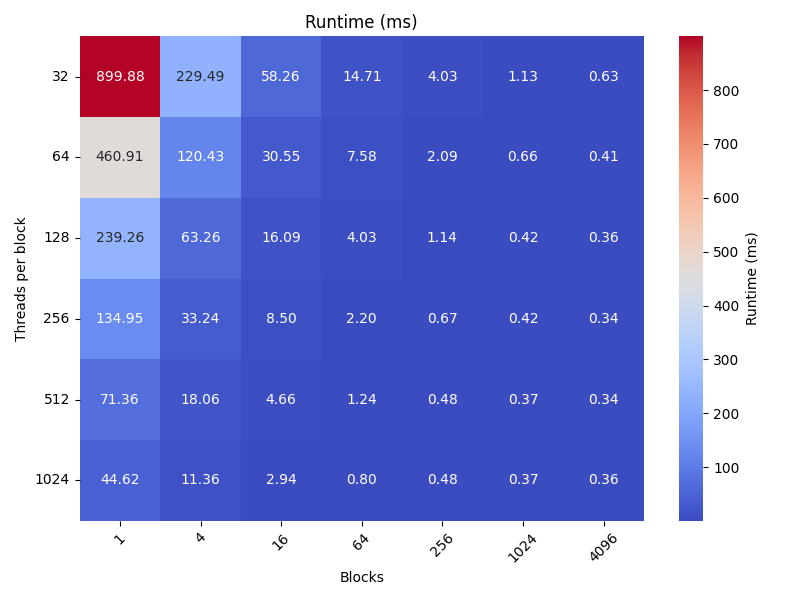
\includegraphics[width=1.0\linewidth]{images/Runtime (ms).png}
    \caption{Heatmap for Runtime (ms)}
    \label{fig:runtime_heatmap}
\end{figure}


Figure~\ref{fig:occupancy_heatmap} shows that Achieved Occupancy improves significantly with larger thread block sizes and a higher number of threads per block. With more threads per block, more warps are available, enabling greater concurrent warp scheduling. Consequently, occupancy increases as threads per block increase. However, increasing the number of thread blocks does not enhance occupancy until the count reaches 256, as the GPU contains 108 SMs (see Section~\ref{subsec:computational-platform-and-software-environment}). Below this threshold, each SM handles only one thread block, limiting occupancy gains. Beyond this point, additional thread blocks can be allocated per SM, further increasing occupancy.

\begin{figure}[htbp]
    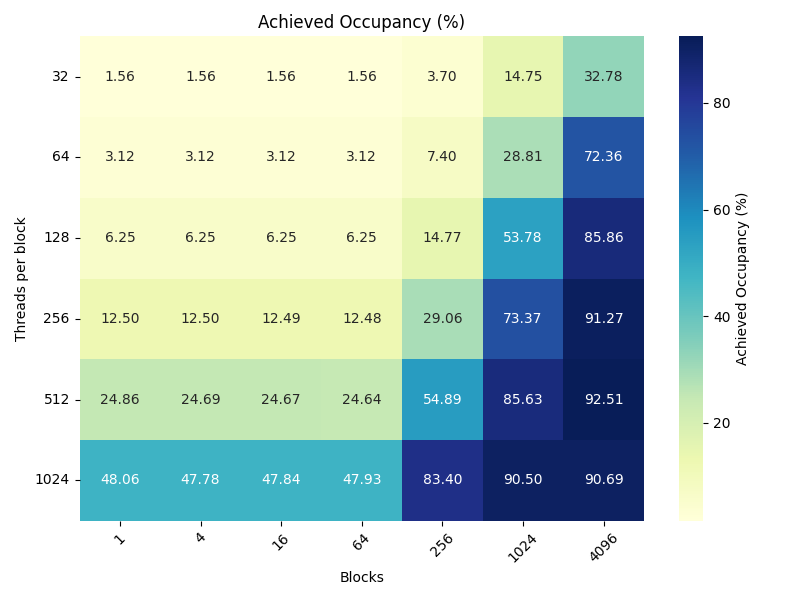
\includegraphics[width=1.0\linewidth]{images/Achieved Occupancy.png}
    \caption{Heatmap for Achieved Occupancy (\%)}
    \label{fig:occupancy_heatmap}
\end{figure}


Figure~\ref{fig:memory_bandwidth_heatmap} reveals that the Percentage of Peak Sustained Memory Bandwidth is higher with larger threads per block and increased thread block counts, indicating a positive correlation with the total thread count. However, maximum memory bandwidth utilization does not occur at the highest configuration of (T, B) = (1024, 4096). Instead, configurations such as (T, B) = (512, 4096) and others with slightly lower counts (e.g., (512, 1024) or (256, 4096)) perform better. This discrepancy is likely due to the image size used in the experiment (\(7112 \times 5146\)), where each thread is assigned 8 or 9 pixels when (T, B) = (1024, 4096). In this setup, threads assigned 8 pixels complete their tasks faster and must wait for threads assigned 9 pixels, leading to idle time. This overhead becomes significant when fewer pixels are assigned per thread, reducing the efficiency gains from the higher thread count as idle time increases.

\begin{figure}[htbp]
    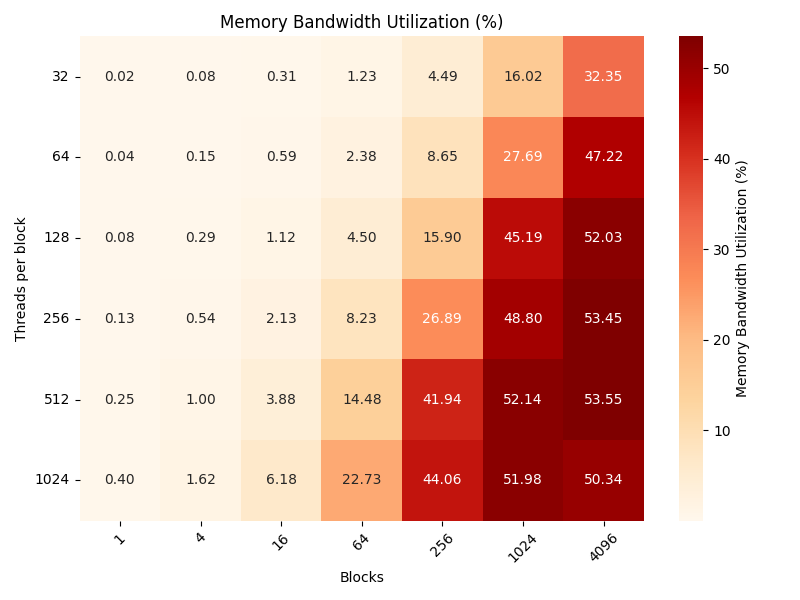
\includegraphics[width=1.0\linewidth]{images/Memory Bandwidth Utilization.png}
    \caption{Heatmap for Percentage of Peak Sustained Memory Bandwidth (\%)}
    \label{fig:memory_bandwidth_heatmap}
\end{figure}